\chapter{Project Planning}
\label{Chapter4}

%TODO: Compararho amb el real

\section{Schedule}
\subsection{Estimated project duration}
For this project there have been estimated 450 hours of work, starting on \textbf{19th of February} and ending on \textbf{23rd of June}.\\

\subsection{Considerations}
The original plan could be modified to be adapted to deviations. Agile methodology implies that some new requirements can appear which could modify the planning. It is hard to do a realistic planning with Agile methodology because the iteration's requirements are not fully known until the Planning stage.\\

Because this project will be developed sequentially by only one person, the realization of a PERT diagram has been discarded. Nevertheless, some part of the documentation will be done in parallel.

\section{Resources}
For the development of this project, three types of resources will be needed.
\subsection{Human Resources}
\begin{itemize}
	\item One person working 20 hours per week until the finalization of the project.
\end{itemize}
\subsection{Material Resources}
\begin{itemize}
	\item Lenovo IdeaPad U330T\\
	This laptop will be used to write the documentation and develop the project.
\end{itemize}
\subsection{Software Resources}
\begin{itemize}
	\item Trello: Web application to manage project tasks.
	\item teXstudio: LateX editor to write all the documentation.
	\item e-mail: Communication tool used to contact the supervisor. 
	\item Atom: Text editor to write the code.
	\item Git: VCS to backup and keep tracking of the project.
	\item C++: Language used for the development.
	\item PBLib: C++ library for Pseudo-Boolean encodings.
	\item CLion: Code editor focused on C++.
	\item Google Test: Unit testing framework for C++ developed by Google.
\end{itemize}

\section{Project Planning}

\subsubsection{GEP}
This task corresponds to the work done during the GEP course. This task has not any dependency but the work done will be used for the final documentation.\\

The estimated time for this stage is 70 hours.
\subsubsection{Initial Stage}
This stage will be used for defining the requisites to accomplish, the architecture of the software and refactor the previous code. Also, the required tools will be installed. \\

The estimated time for this stage is 90 hours.
\subsubsection{Iterations}
Because Agile methodology will be followed, the project has been divided into iterations. There will be a total of 3 iterations: Pseudo-Boolean minimization, Timeout strategies, and Multithreading, being this last one optional. \\

For each iteration, 80h of work are estimated.
\paragraph{Planning\\}
This stage will be used for defining the scope of the iteration and goals.\\

This stage will be 10 hours long.
\paragraph{Development and TDD\\}
In this stage, the iteration will be developed and tested.\\

This stage will be 60 hours long.
\paragraph{Finalization\\}
In this stage, all possible bugs will be solved and feedback from the supervisor will be taken.\\

This stage will be 10 hours long.


\subsubsection{Final Stage}
Here, all the development will be finished and it will be used for finishing all the documentation and prepare the final presentation.\\

This stage will take 50 hours.

\subsection{Gantt Diagram}
\begin{figure}[hbtp] 
	\centering
	\makebox[\textwidth]{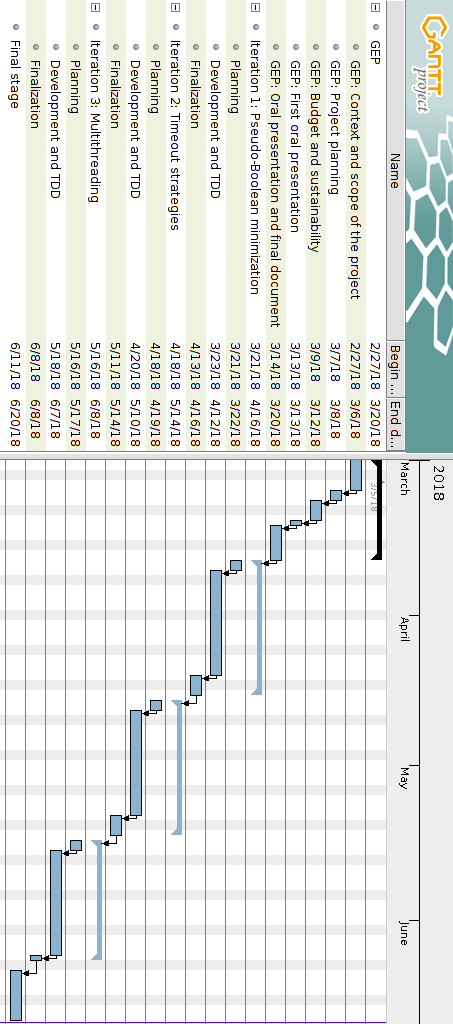
\includegraphics[height=.60\paperheight]{Figures/GanttTable2.png}}
	\caption{Gantt diagram of the project}
	\label{GanttDiagram}
\end{figure}


\section{Alternatives and Action Plans}
Because of using an Agile methodology, the project functionalities can be easily adapted during the development. \\

\subsection{Potential deviations}
\subsubsection{Incorrect estimations}
It could be that the purposed estimations are not correct and be underestimated or overestimated. In the first case, if some iteration takes less time than expected, the next iteration will be started immediately. On the other case, if an iteration takes more time than expected, more hours will be added, for example, weekend hours. If even with this countermeasures the iteration is delaying the project some optional improvements will be discarded in order to guarantee the main functionalities and the project would be finished before the deadline. 
The effect on the resources would be more electricity consumed by the laptop on the added hours. 

\subsubsection{Summer internship}

The deadline for this project is the 23rd of June. 
I have applied for a CERN internship from 4th of June until 31st of August. 

In case of being accepted into the program, the final stage would have to be done during the internship. Since the final stage is for doing the final document and the final presentation, it can be lightened by paralleling part of its work during other stages.

The duration of the project is not affected because the only thing that would be done is a different distribution of the work. For the same reason, it would not have any effect on the resources.

\subsubsection{Compatibility issues}

As explained before, in section X, PBLib could cause some compatibility issues with the existing software which works with another library, Cudd. 
If this happens, in the best situation some hours will be spent fixing this issue or finding a substitute. In the worst situation, the functionalities of PBLib would have to be implemented which would take a lot of time. The project duration could be affected but it would be always finished before the deadline using weekend hours. The resources which will be used in addition is more electricity consumed by the laptop.

\subsubsection{Base project code quality}
The existing project could have some quality issues and be a source of bugs which would cause a lot of delays. For this reasons, and as s explained in section Y, the first stage of this project will be focused on assuring quality code of the existing project.  The project duration would not be affected because part of the first stage is focused on that guaranteeing project finalization.\\\\\\

As explained in each potential deviation, the priority is to finish the project before the deadline.  As said, extra-hours from the weekend can be used to work on the project to accomplish all the objectives. If even these hours are not enough, then the optional objective \emph{Multithreading} will not be realized. 